\section{Evaluations}
\label{sec:eval}
In this section, we first give a statistical overview of AliCoCo.
Next we present experimental evaluations for five main technical modules 
during the construction of AliCoCo.

\subsection{Overall Evaluation}

\tabref{tab:data} shows the statistics of AliCoCo.
%~\footnote{We attempt to release an API for visiting AliCoCo in the near future.}.
There are $2,853,276$ primitive concepts and $5,262,063$ e-commerce concepts in total at the time of writing.
There are hundreds of billions of relations in AliCoCo, including $131,968$ isA relations within \textit{Category} in the layer of primitive concepts and $22,287,167$ isA relations in the layer of e-commerce concepts.
For over $3$ billion items in Alibaba, $98\%$ of them are linked to AliCoCo.
Each item is associated with $14$ primitive concepts and $135$ e-commerce concepts on average.
Each e-commerce concept is associated with $74,420$ items on average.
The number of relations between e-commerce concept layer and primitive concept layer is $33,495,112$.

AliCoCo is constructed semi-automatically.
For those nodes and relations mined by models, 
we will randomly sample part of data and ask human annotators to label.
Only if the accuracy achieves certain threshold,
the mined data will be added into AliCoCo to ensure the quality.
Besides, for those dynamic edges (associated with items),
we monitor the data quality regularly.


\begin{table}[th]
%	\centering
	\small
	\begin{tabular}{|l|l|l|l|}
		\hline
		\multicolumn{4}{|l|}{\textbf{Overall}} \\ 
		\hline
		\multicolumn{2}{|l|}{\# Primitive concepts} &
		\multicolumn{2}{l|}{2,853,276}  \\
		\hline
		\multicolumn{2}{|l|}{\# E-commerce concepts} &  
		\multicolumn{2}{l|}{5,262,063}  \\ 
		\hline
		\multicolumn{2}{|l|}{\# Items} &
		\multicolumn{2}{l|}{> 3 billion} \\ 
		\hline
		\multicolumn{2}{|l|}{\# Relations} &
		\multicolumn{2}{l|}{> 400 billion} \\ 
		\hline
		\hline
		\multicolumn{4}{|l|}{\textbf{Primitive concepts}} \\ 
		\hline
		\# Audience &\# Brand &\# Color &\# Design  \\
		\cline{1-4}
		15,168 & 879,311 & 4,396 & 744 \\
		\cline{1-4}
		\# Event & \# Function & \# Category &\# IP  \\
		\cline{1-4}
		 18,400 & 16,379 & 142,755 & 1,491,853
		  \\
		\cline{1-4}
		\# Material & \# Modifier & \# Nature &\# Organization  \\
		\cline{1-4}
		 4,895 & 106 & 75 & 5,766 \\
		\cline{1-4}
		\# Pattern & \# Location & \# Quantity &\# Shape  \\
		\cline{1-4}
		 486 & 267,359 & 1,473 & 110 \\
		\cline{1-4}
		\# Smell & \# Style & \# Taste &\# Time  \\
		\cline{1-4}
		 9,884 & 1,023 & 138 & 365 \\
		\hline
		\hline
		\multicolumn{4}{|l|}{\textbf{Relations}} \\ 
		\hline
		\multicolumn{2}{|l|}{\# IsA in primitive concepts} &
		\multicolumn{2}{l|}{131,968 (only in \textit{Category})}  \\
		\hline
		\multicolumn{2}{|l|}{\# IsA in e-commerce concepts} &
		\multicolumn{2}{l|}{22,287,167}  \\
		\hline
		\multicolumn{2}{|l|}{\# Item - Primitive concepts} &
		\multicolumn{2}{l|}{21 billion}  \\
		\hline
		\multicolumn{2}{|l|}{\# Item - E-commerce concepts} &
		\multicolumn{2}{l|}{405 billion}  \\
		\hline
		\multicolumn{2}{|l|}{\# E-commerce - Primitive cpts} &
		\multicolumn{2}{l|}{33,495,112}  \\
		\hline
		%		\bottomrule
	\end{tabular}
	\caption{Statistics of AliCoCo at the time of writing.}
	\label{tab:data}
\end{table}

To evaluate the coverage of actual shopping needs of our customers, we sample $2000$ search queries at random and manually rewrite them into coherent word sequences, then we search in AliCoCo to calculate the coverage of those words. 
We repeat this procedure every day, in order to detect new trends of user needs in time. 
AliCoCo covers over $75\%$ of shopping needs on average in continuous $30$ days, while this number is only $30\%$ for the former ontology mentioned in \secref{sec:intro}.


\subsection{Primitive Concept Mining}
\label{sec:eval_mining}
After defining $20$ different domains in the taxonomy,
we quickly enlarge the size of primitive concepts by introducing knowledges from several existing structured or semi-structured knowledge bases in general-purpose domain.
During this step, vocabulary sizes of domains such as $Location$, $Organization$ and $IntellectulProperty$ can be quickly enlarged.
Other domains are for e-commerce use, and we mainly leverage the existing e-commerce semi-structured data: CPV, since most of $Property$s can be matched to our domains such as $Brand$, $Color$, $Material$, etc.

After rule based alignments and cleaning, 
around $2M$ primitive concepts can be drawn from multiple sources.
We adopt the idea of distant supervision to
generate a large amount of training samples,
in order to mine new concepts.
We use a dynamic programming algorithm of max-matching to match words in the text corpora and then assign each word with its domain label in IOB scheme using existing primitive concepts. We filter out sentences whose matching result is ambiguous and only reserve those that can be perfectly matched (all words can be tagged by only one unique label) as our training data.
We generate around $6M$ training data in this way.
In each epoch of processing $5M$ sentences, 
our mining model is able to discover around $64K$ new candidate concepts on average.
After manually checking the correctness by crowdsourcing services, 
around $10K$ correct concepts can be added into our vocabulary in each round.
The mining procedure is continuously running, 
and the total number of primitive concepts from all $20$ domains 
is $2,758,464$ at the time of writing.









\subsection{Hypernym Discovery}

In order to organize all the primitive concepts into a fine-grained taxonomy,
we propose an active learning framework to iteratively 
discover isA relation between different primitive concepts.
To demonstrate the superior of our framework, 
we perform several experiments on a ground truth dataset collected after the taxonomy is constructed.
We randomly sample 3,000 primitive concepts in the class of ``\textit{Category}'' which have at least one hypernym, and retrieve 7,060 hyponym-hypernym pairs as positive samples.
We split the positive samples into training / validation / testing sets (7:2:1).
The search space of hypernym discovery is actually the whole vocabulary, 
making the number and quality of negative samples very important in this task.
The negative samples of training and validation sets are automatically generated from positive pairs
by replacing the hypernym of each pair with a random primitive concept from ``\textit{Category}'' class.
In the following experiments, mean average precision (MAP), mean reciprocal rank (MRR) and precision at rank 1 (P@1) are used as evaluation metrics. 

To verify the appropriate number of negative samples for each hyponym during training,
we perform an experiment shown in \figref{fig:isa}(left), 
where $N$ in x-axis represents the ratio of negative samples over positive samples for each hyponym.
The results indicate different size of negative samples influence the performance differently.
As $N$ gradually increases, the performance improves and achieves best around $100$.
Thus, we construct the candidate training pool in the following active learning experiment with a size of $500,000$.

\begin{figure}[th]
	\centering
	\epsfig{file=figures/isa.eps, width=\columnwidth}
	\caption{Left: the influence of different negative sample sizes in hypernym discovery on test set. Right: the best performance of different sampling strategies in active learning.}
	\label{fig:isa}
\end{figure}

\tabref{tab:isa} shows experimental results of different sampling strategies during our active learning framework, 
where $Random$ means training using the whole candidate pool without active learning.
We set the select data size $K$ as $25,000$ in each iteration as mentioned in \secref{sec:isa}.
When it achieves similar MAP score in four active learning strategies,
we can find that all the active learning sampling strategies can reduce labeled data to save considerable manual efforts.
UCS is the most economical sampling strategy, which only needs $325k$ samples, reducing $35\%$ samples comparing to random strategy.
It indicates that high confident negative samples are also important in the task of hypernym discovery.

\begin{table}[th]
	\centering
	%\scriptsize
	\begin{tabular}{l|c|c|c|c|c}
		\hline
		Strategy & Labeled Size &  MRR & MAP & P@1 & Reduce \\
		\hline
		Random & 500k & 58.97 & 45.30 & 45.50 & - \\
		US  & 375k &  59.66 & 45.73 & 46.00 & 150k\\
		CS & 400k &  58.96 & 45.22 & 45.30 & 100k\\
		UCS  & 325k &  59.87 & 46.32 & 46.00 & 175k \\
		\hline
	\end{tabular}
	\caption{Experimental results of different sampling strategy in hypernym discovery.}
	\label{tab:isa}
\end{table}

In \figref{fig:isa} (right), 
we show the best performance of each sampling strategies during the whole training procedure.
UCS outperforms other three strategies and achieves a highest MAP of $48.82\%$, showing the importance of selecting the most valuable samples during model training.






\subsection{E-commerce Concept Classification}

In this subsection,
we mainly investigate how each component of our model influences the performance in the task of judging whether a candidate e-commerce concept satisfy the criteria or not (\secref{sec:classification}).

We randomly sample a large portion of e-commerce concepts from the candidate set and ask human annotators to label \footnote{The annotation task lasts for several months until we get enough training samples.}. The final dataset consists of $70k$ samples (positive: negative= 1: 1). Then we split the dataset into 7:1:2 for training, validation and testing. 

\begin{table}[th]
	\centering
	%\scriptsize
	\begin{tabular}{l|c}
		\hline
		Model & Precision   \\
		\hline
		Baseline (LSTM + Self Attention) & 0.870 \\
		+Wide  & 0.900 \\
		+Wide \& BERT & 0.915 \\
		+Wide \& BERT \& Knowledge & \textbf{0.935} \\
		\hline 
	\end{tabular}
	\caption{Experimental results in shopping concept generation. }
	\label{tab:concept}
\end{table}

Results of ablation tests are shown in \tabref{tab:concept}.
Comparing to the baseline, which is a base BiLSTM with self attention architecture, adding wide features such as different syntactic features of concept improves the precision by $3\%$ in absolute value.
When we replace the input embedding with BERT output,
the performance improves another $1.5\%$, 
which shows the advantage of rich semantic information
encoded by BERT.
After introducing external knowledge into our model,
the final performance reaches to $0.935$, improving by a relative gain of $7.5\%$ against the baseline model, indicating that leveraging external knowledge benefits commonsense reasoning on short concepts.




\subsection{E-commerce Concept Tagging}

To associate those e-commerce concepts which are directly mined from text corpus to the layer of primitive concepts,
we propose a text-augmented NER model with fuzzy CRF mentioned in \secref{sec:tagging}
to link an e-commerce concept to its related primitive concepts.
We randomly sample a small set ($7,200$) of e-commerce concepts
and ask human annotators to label the correct class labels for each primitive concepts within the e-commerce concepts.
To enlarge the training data, 
we use the similar idea of distant supervision mentioned in \secref{sec:eval_mining}
to automatically generate $24,000$ pairs of data.
Each pair contains a compound concept and its corresponding gold sequence of domain labels.
We split $7,200$ pairs of manually labeled data into 
$4,800/1,400/1,000$ for training, validation and testing.
$24,000$ pairs of distant supervised data are added into training set to help learn a more robust model.

\begin{table}[th]
	\centering
	%\scriptsize
	\begin{tabular}{l|c|c|c}
		\hline
		Model & Precision &  Recall & F1  \\
		\hline
		Baseline & 0.8573 & 0.8474 &	0.8523 \\
		+Fuzzy CRF  & 0.8731 &  0.8665 & 0.8703 \\
		+Fuzzy CRF \& Knowledge & \textbf{0.8796} &  \textbf{0.8748} & \textbf{0.8772} \\
		\hline
	\end{tabular}
	\caption{Experimental results in shopping concept tagging.}
	\label{tab:linking}
\end{table}

Experimental results are shown in \tabref{tab:linking}.
Comparing to baseline which is a basic sequence labeling model with Bi-LSTM and CRF, 
adding \textit{fuzzy CRF} improves 1.8\% on F1, 
which indicates such multi-path optimization in CRF layer actually contributes to disambiguation.
Equipped with external knowledge embeddings to further enhance the textual information, 
our model continuously outperform to $0.8772$ on F1.
It demonstrates that introducing external knowledge can benefit tasks dealing with short texts with limited contextual information.

\subsection{Concept-Item Semantic Matching}


In this subsection,
we demonstrate the superior of our semantic matching model
for the task of associating e-commerce concepts with billion of items in Alibaba.
We create a dataset with a size of $450m$ samples, among which $250m$ are positive pairs and $200m$ are negative pairs.
The positive pairs comes from strong matching rules and user click logs of the running application on Taobao mentioned in \secref{sec:intro}.
Negative pairs mainly comes from random sampling.
%共392个不同query,通过人工标注20w正、20w负,总计40w
For testing, we randomly sample $400$ e-commerce concepts,
and ask human annotator to label based on a set of candidate pairs.
In total, we collect $200k$ positive pairs and $200k$ negative pairs as testing set.

\begin{table}[th]
	\centering
	%\scriptsize
	\begin{tabular}{l|c|c|c}
		\hline
		Model & AUC & F1 & P@10   \\
		\hline
		BM25 & - & - & 0.7681 \\
		DSSM \cite{huang2013learning}  & 0.7885 & 0.6937 & 0.7971  \\
		MatchPyramid \cite{pang2016text} & 0.8127 & 0.7352 & 0.7813  \\
		RE2 \cite{yang2019simple} \ & 0.8664 & 0.7052 & 0.8977  \\
		\hline
		Ours & 0.8610 & 0.7532 & 0.9015  \\
		Ours + Knowledge & \textbf{0.8713} & \textbf{0.7769} & \textbf{0.9048}  \\
		\hline 
	\end{tabular}
	\caption{Experimental results in semantic matching between e-commerce concepts and items.}
	\label{tab:matching}
\end{table}

\tabref{tab:matching} shows the experimental result, 
where F1 is calculated by setting a threshold of $0.5$.
Our knowledge-aware deep semantic matching model outperforms all the baselines in terms of AUC, F1 and Precision at $10$,
showing the benefits brought by external knowledge.
To further investigate how knowledge helps, 
we dig into cases. Using our base model without knowledge injected,
the matching score of concept ``中秋节礼物 (Gifts for Mid-Autumn Festival)'' and item ``老式大月饼共800g云南特产荞三香大荞饼荞酥散装多口味 (Old big moon cakes 800g Yunnan...)'' is not confident enough to associate those two, since the texts of two sides are not similar.
After we introduce external knowledge for ``中秋节 (Mid-Autumn Festival)'' such as ``中秋节自古便有赏月、吃月饼、赏桂花、饮桂花酒等习俗。(It is a tradition for people to eat moon cakes in Mid-Autumn...)'', 
the attention score for ``中秋节 (Mid-Autumn Festival)'' and ``月饼 (moon cakes)'' increase to bridge the gap of this concept-item pair.
  
